%!TEX root = ../Thesis.tex
%% Basierend auf TeXnicCenter-Vorlage von Mark Müller
%%                      Willi Nüßer
%%                      Waldemar Penner
%%                      Ulrich Reus
%%                      Frank Plass
%%                      Oliver Tribeß
%%                      Daniel Hintze
%%%%%%%%%%%%%%%%%%%%%%%%%%%%%%%%%%%%%%%%%%%%%%%%%%%%%%%%%%%%%%%%%%%%%%%

% Wählen Sie die Optionen aus, indem Sie % vor der Option entfernen
% Dokumentation des KOMA-Script-Packets: scrguide

%%%%%%%%%%%%%%%%%%%%%%%%%%%%%%%%%%%%%%%%%%%%%%%%%%%%%%%%%%%%%%%%%%%%%%%
%% Optionen zum Layout des Artikels                                  %%
%%%%%%%%%%%%%%%%%%%%%%%%%%%%%%%%%%%%%%%%%%%%%%%%%%%%%%%%%%%%%%%%%%%%%%%
\documentclass[%
paper=A4,         % alle weiteren Papierformat einstellbar
fontsize=11pt,    % Schriftgröße (12pt, 11pt (Standard))
BCOR12mm,         % Bindekorrektur, bspw. 1 cm
DIV14,            % breiter Satzspiegel
parskip=half*,    % Absatzformatierung s. scrguide 3.1
headsepline,      % Trennline zum Seitenkopf
%footsepline,     % Trennline zum Seitenfuß
%normalheadings,  % Überschriften etwas kleiner (smallheadings)
listof=totoc,     % Tabellen & Abbildungsverzeichnis ins Inhaltsverzeichnis
%bibtotoc,        % Literaturverzeichnis im Inhalt
%draft            % Überlangen Zeilen in Ausgabe gekennzeichnet
footinclude=false,% Fußzeile in die Satzspiegelberechnung einbeziehen
headinclude=true, % Kopfzeile in die Satzspiegelberechnung einbeziehen
final             % draft beschleunigt die Kompilierung
]
{scrartcl}

%\setuptoc{toc}{totoc} % Inhaltsverzeichnis ins Inhaltsverzeichnis

% Neue Deutsche Rechtschreibung und Deutsche Standardtexte
\usepackage[ngerman]{babel}

% Umlaute können verwendet werden
\usepackage[utf8]{inputenc}

% Echte Umlaute
\usepackage[T1]{fontenc}

% Latin Modern Font, Type1-Schriftart für nicht-englische Texte
\usepackage{lmodern}

% 1/2-zeiliger Zeilenabstand
\usepackage[onehalfspacing]{setspace}

% Für die Defenition eigener Kopf- und Fußzeilen
\usepackage{fancyhdr}

% Für die Verwendung von Grafiken
\usepackage[pdftex]{graphicx}

% Bessere Tabellen
\usepackage{tabularx}

% Für die Befehle \toprule, \midrule und \bottomrule, z.B. in Tabellen
\usepackage{booktabs}

% Erlaubt die Benutzung von Farben
\usepackage{color}

% Verbessertes URL-Handling mit \url{http://...}
\usepackage{url}

% Listen ohne Abstände \begin{compactlist}...\end{compactlist}
\usepackage{paralist}

% Ausgabe der aktuellen Uhrzeit für die Draft-Versionen
\usepackage{datetime}

% Deutsche Anführungszeichen
\usepackage[babel,german=quotes]{csquotes}

% Konfiguration der Abbildungs- und Tabellenbezeichnungen
\usepackage[format=hang, font={footnotesize, sf}, labelfont=bf, justification=raggedright,singlelinecheck=false]{caption}

% Verbessert die Lesbarkeit durch Mikrotypografie
\usepackage[activate={true,nocompatibility},final,tracking=true,kerning=true,spacing=true,factor=1100,stretch=10,shrink=10]{microtype}

% Zitate und Quellenverzeichnis
\usepackage[
bibstyle=authoryear,
citestyle=authoryear-fhdw,
firstinits=false,         % false = Vornamen werden ausgeschrieben
natbib=true,
urldate=long,             % "besucht am" - Datum
%url=false,
date=long,
dashed=false,
maxcitenames=3,           % max. Anzahl Autorennamen in Zitaten
maxbibnames=99,           % max. Anzahl Autorennamen im Quellenverzeichnis
%backend=bibtex           % Ggf. für ältere Distributionen bibtex verwenden
backend=biber
]{biblatex}

%Namen nach Schema "Nachname, Vorname" für alle Autoren
\DeclareNameAlias{sortname}{last-first}

%benutze "et al." statt "u.a."
\DefineBibliographyStrings{ngerman}{
andothers = {{et\,al\adddot}},
}

% Bibliograpthy
\bibliography{library/library}

% Keine Einrückung bei einem neuen Absatz
\parindent 0pt

% Ebenentiefe der Nummerierung
\setcounter{secnumdepth}{3}

% Gliederungstiefe im Inhaltsverzeichnis
\setcounter{tocdepth}{3}

% Tabellen- und Abbildungsverzeichnis mit Bezeichnung:
\usepackage[titles]{tocloft}

% Sourcecode-Listings
\usepackage{listings}

% Bestimmte Warnungen unterdrücken
% siehe http://tex.stackexchange.com/questions/51867/koma-warning-about-toc
\usepackage{scrhack}

%% http://tex.stackexchange.com/questions/126839/how-to-add-a-colon-after-listing-label
\makeatletter
\begingroup\let\newcounter\@gobble\let\setcounter\@gobbletwo
\globaldefs\@ne \let\c@loldepth\@ne
\newlistof{listings}{lol}{\lstlistlistingname}
\endgroup
\let\l@lstlisting\l@listings
\makeatother

\renewcommand*\cftfigpresnum{Abbildung~}
\renewcommand*\cfttabpresnum{Tabelle~}
\renewcommand*\cftlistingspresnum{Listing~}
\renewcommand{\cftfigaftersnum}{:}
\renewcommand{\cfttabaftersnum}{:}
\renewcommand{\cftlistingsaftersnum}{:}
\settowidth{\cftfignumwidth}{\cftfigpresnum 99~\cftfigaftersnum}
\settowidth{\cfttabnumwidth}{\cfttabpresnum 99~\cftfigaftersnum}
\settowidth{\cftlistingsnumwidth}{\cftlistingspresnum 99~\cftfigaftersnum}
\setlength{\cfttabindent}{1.5em}
\setlength{\cftfigindent}{1.5em}
\setlength{\cftlistingsindent}{1.5em}

\renewcommand\lstlistlistingname{Listingverzeichnis}

% Style für Kopf- und Fußzeilenfelder
\pagestyle{fancy}
\fancyhf{}
\fancyhead[R]{\leftmark}
\fancyfoot[R]{\thepage}
\renewcommand{\sectionmark}[1]{\markboth{#1}{#1}}
\fancypagestyle{plain}{}

% Macro für Quellenangaben unter Abbildungen und Tabellen
\newcommand{\source}[1]{{\vspace{-1mm}\\\footnotesize\textsf{\textbf{Quelle:}} \textsf{#1}\par}}

% Anpassungen der Formatierung an Eclipse-Aussehen
% http://jevopi.blogspot.de/2010/03/nicely-formatted-listings-in-latex-with.html
%\definecolor{sh_comment}{rgb}{0.12, 0.38, 0.18 } %adjusted, in Eclipse: {0.25, 0.42, 0.30 } = #3F6A4D
%\definecolor{sh_keyword}{rgb}{0.37, 0.08, 0.25}  % #5F1441
%\definecolor{sh_string}{rgb}{0.06, 0.10, 0.98} % #101AF9
% Für Druckausgabe sollte alles schwarz sein
\definecolor{sh_comment}{rgb}{0.0, 0.0, 0.0 }
\definecolor{sh_keyword}{rgb}{0.0, 0.0, 0.0 }
\definecolor{sh_string}{rgb}{0.0, 0.0, 0.0 }

\lstset{ %
language=Java,
basicstyle=\small\ttfamily,
fontadjust,
xrightmargin=1mm,
xleftmargin=5mm,
tabsize=2,
columns=flexible,
showstringspaces=false,
rulesepcolor=\color{black},
showspaces=false,showtabs=false,tabsize=2,
stringstyle=\color{sh_string},
keywordstyle=\color{sh_keyword}\bfseries,
commentstyle=\color{sh_comment}\itshape,
captionpos=t,
lineskip=-0.3em
}

%\makeatletter
%\def\l@lstlisting#1#2{\@dottedtocline{1}{0em}{1.5em}{\lstlistingname\space{#1}}{#2}}
%\makeatother

% Anhangsverzeichnis
\usepackage[nohints]{minitoc} %Anhangsverzeichnis

\makeatletter
\newcounter{fktnr}\setcounter{fktnr}{0}
\newcounter{subfktnr}[fktnr]\setcounter{subfktnr}{0}

\renewcommand\thesubfktnr{\arabic{fktnr}.\arabic{subfktnr}}
\newcounter{anhangcounter}
\newcommand{\blatt}{\stepcounter{anhangcounter}}

\newcommand{\anhang}[1]{\setcounter{anhangcounter}{0}\refstepcounter{fktnr}
\addcontentsline{fk}{subsection}{Anhang~\thefktnr: \hspace*{1em}#1}
\subsection*{{Anhang~\thefktnr \hspace*{1em} #1 \hspace*{-1em}}}
}

\newcommand{\subanhang}[1]{\setcounter{anhangcounter}{0}\refstepcounter{subfktnr}
\addcontentsline{fk}{subsubsection}{Anhang~\thesubfktnr: \hspace*{1em}#1}
\subsubsection*{{Anhang~\thesubfktnr \hspace*{1em} #1 \hspace*{-1em}}}
}

\newcommand{\anhangsverzeichnis}{\mtcaddsection{\subsection*{Anhangsverzeichnis \@mkboth{FKT}{FKT}}}\@starttoc{fk}\newpage}

% Links im PDF
\usepackage[pdfpagemode={UseOutlines}, plainpages=false,breaklinks=true,pdfpagelabels]{hyperref}

% Abkürzungsverzeichnis
\usepackage[acronym,         % create list of acronyms
nonumberlist,
toc,
section,
nomain,          % don't need main glossary for this example
hyperfirst=false,% don't hyperlink first use
sanitize=none    % switch off sanitization as description
]{glossaries}
\newglossarystyle{mylist}{%
\glossarystyle{long}% base this style on the list style
\renewcommand*{\glossaryentryfield}[5]{%
\glsentryitem{##1}\textbf{##2} & ##3 \\}%
}

% Verbessert das Referenzieren von Kapiteln, Abbildungen etc.
\usepackage[german,capitalise]{cleveref}

\input{config/Abkuerzungen}
\makeglossaries\makeglossaries

\usepackage{float}

%%%%%%%%%%%%%%%%%%%%%%%%%%%%%%%%%%%%%%%%%%%%%%%%%%%%%%%%%%%%%%%%%%%%%%%
%% Parameter - Hier auf die eigene Arbeit anpassen
%%%%%%%%%%%%%%%%%%%%%%%%%%%%%%%%%%%%%%%%%%%%%%%%%%%%%%%%%%%%%%%%%%%%%%%

\newcommand{\dokumententyp}{Schriftliche Ausarbeitung}
\newcommand{\abgabedatum}{\today}
\newcommand{\ort}{Paderborn}
\newcommand{\koorperationsunternehmen}{\enquote{Geile Typen GmbH}}
\newcommand{\dokumententitel}{Dokumentation Anwendung \enquote{Wettersensoren}\\ im Rahmen des Moduls \enquote{AWE2}}
\newcommand{\dokumentenautor}{Jonathan Brockhausen, Philipp Röring, Julius Figge}
\newcommand{\dokumentenautoradress}{}
\newcommand{\dokumentenpruefer}{Florian Wortmann}
\newcommand{\studiengang}{Angewandte Informatik B.Sc.}

%%%%%%%%%%%%%%%%%%%%%%%%%%%%%%%%%%%%%%%%%%%%%%%%%%%%%%%%%%%%%%%%%%%%%%%

\hypersetup{
colorlinks=false,
pdfborder={0 0 0},
pdftitle=\dokumententitel,
pdfauthor=\dokumentenautor
}

\begin{document}

    % Römische Seitennummerierung
    \pagenumbering{Roman}

    %%%%%%%%%%%%%%%%%%%%%%%%%%%%%%%%%%%%%%%%%%%%%%%%%%%%%%%%%%%%%%%%%%%%%%%
    %% Titelseite
    %%%%%%%%%%%%%%%%%%%%%%%%%%%%%%%%%%%%%%%%%%%%%%%%%%%%%%%%%%%%%%%%%%%%%%%

    %!TEX root = ../Thesis.tex

\begin{titlepage}

    \begin{center}


        
\includegraphics[scale=1.20]{img/fhdw}\\

        \vspace{.7cm}

        \Huge{\bfseries\dokumententyp}

        ~\vspace{.5cm}\\

        \LARGE{\dokumententitel}

        ~\vspace{1.2cm}\\


        \large{

        Prüfer:\vspace{1mm}\\

        \dokumentenpruefer

        \vspace{1cm}

        Erstellt von:\\\vspace{1mm}

        \dokumentenautor\\

        \dokumentenautoradress

        \vspace{1cm}

        Studiengang:\vspace{1mm}\\

        \studiengang

        \vspace{1cm}

        Eingereicht am:\vspace{1mm}\\

        \abgabedatum

        }

    \end{center}


\end{titlepage}



    %%%%%%%%%%%%%%%%%%%%%%%%%%%%%%%%%%%%%%%%%%%%%%%%%%%%%%%%%%%%%%%%%%%%%%%
    %% Draft-Einstellungen
    %%
    %% Für die finale Version auskommentieren!
    %%%%%%%%%%%%%%%%%%%%%%%%%%%%%%%%%%%%%%%%%%%%%%%%%%%%%%%%%%%%%%%%%%%%%%%
    %    \fancyhead[L]{\color{red} Stand: \today~-~\currenttime}

    %%%%%%%%%%%%%%%%%%%%%%%%%%%%%%%%%%%%%%%%%%%%%%%%%%%%%%%%%%%%%%%%%%%%%%%
    %% Verzeichnisse
    %%%%%%%%%%%%%%%%%%%%%%%%%%%%%%%%%%%%%%%%%%%%%%%%%%%%%%%%%%%%%%%%%%%%%%%


    % Sperrvermerk
    %\include{chapter/Sperrvermerk}

    % Inhaltsverzeichnis
    \tableofcontents

    % Abkürzungsverzeichnis
    \printglossary[type=\acronymtype, style=mylist, title=Abkürzungsverzeichnis, toctitle=Abkürzungsverzeichnis]\newpage
    \setcounter{table}{0} % printglossary erzeugt eine Tabelle, die die Nummerierung der "echten" Tabellen durcheinander bringt.

    %%%%%%%%%%%%%%%%%%%%%%%%%%%%%%%%%%%%%%%%%%%%%%%%%%%%%%%%%%%%%%%%%%%%%%%
    % Verzeichnisse
    %%%%%%%%%%%%%%%%%%%%%%%%%%%%%%%%%%%%%%%%%%%%%%%%%%%%%%%%%%%%%%%%%%%%%%%

    % Abbildungsverzeichnis
    \fancyhead[R]{\listfigurename}
    \listoffigures\newpage

    % Tabellenverzeichnis
    \fancyhead[R]{\listtablename}
    \listoftables\newpage

    % Quelltextverzeichnis
    \fancyhead[R]{\lstlistlistingname}
    \lstlistoflistings\newpage

    % Kapitelüberschriften für den Arbeitstext
    \fancyhead[R]{\leftmark}

    %%%%%%%%%%%%%%%%%%%%%%%%%%%%%%%%%%%%%%%%%%%%%%%%%%%%%%%%%%%%%%%%%%%%%%%
    %% Inhalt
    %%%%%%%%%%%%%%%%%%%%%%%%%%%%%%%%%%%%%%%%%%%%%%%%%%%%%%%%%%%%%%%%%%%%%%%

    % Arabische Seitennummerierung
    \pagenumbering{arabic}

    % CONTENT
    % (Gliederung)
    % (Pflichtenheft???)
    % Fachkonzept (z.B. fachliche Grundlagen, Abläufe, Use-Cases, GUI-Konzept, Datenmodell, etc.)
    % Projektplan
    % Technisches Konzept (z.B. Architekturen, Objektmodell, E/R-Modell, etc.)
    % Implementierung (z.B. verwendete Bibliotheken, Konzepte, Schnittstellen, etc.)
    % Test (z.B. Komponententest, Integrationstest, Performancetest, Testplan, Testergebnisse, etc. )
    % Projektmanagement(z.B. Projektplan, Soll/Ist-Vergleich, Ressourcenzuordnung)
    % Bewertung und Fazit
    % (Quellenverzeichnis)
    % Anhang

    %TODO konsitenz: Die Anwendung vs. Das Projekt vs. Das Programm
    %TODO Seitenumbrüche fixen
    %TODO All Abbildungen / Tabellen / Listings (ausser im Anhang) brauchen Referenz

    %!TEX root = ../Thesis.tex


\section{Installation}\label{Installation}

\subsection{ESP8266}\label{ESP}
Zur Erfassung der Wetterdaten wird ein BME280 Sensor verwendet, welcher von einem Board mit ESP8266 Mikrocontroller und NodeMCU 1.0 Firmware angesteuert wird. Auf diesem Mikrocontroller kann der Sourcecode \textit{nodemcu.ino} ausgeführt werden. Zum Kompilieren sollte die Arduino IDE verwendet werden, in der zuvor die Treiber für den ESP8266 installiert werden müssen. Dazu muss in den Voreinstellungen folgende Boardverwalter-URL hinzugefügt werden: \textit{\href{http://arduino.esp8266.com/stable/package\_esp8266com\_index.json}{Boardverwalter-URL}}. Darüber hinaus müssen folgende Bibliotheken über die integrierte Bibliotheksverwaltung installiert werden:

\begin{table}[hbt]
    \centering
    \begin{minipage}[t]{.5\textwidth}
        \caption{Verwendete Arduino-Bibliotheken}
        \begin{tabular}{|l|c|}
            \hline
            \textbf{Bibliothek}                       & \textbf{Version} \\
            \hline
            WiFi (by Arduino)                     & 1.2.7            \\
            \hline
            Adafruit BME280 Library (by Adafruit) & 2.1.1            \\
            \hline
            Adafruit Unified Sensor (by Adafruit) & 1.1.4            \\
            \hline
            EasyNTPClient (by Harsha Alva)        & 1.1.0            \\
            \hline
            LinkedList (by Ivan Seidel)           & 1.2.3            \\
			\hline
		\end{tabular}
	\source{Eigene Darstellung}
\label{tab:usedArduinoLibs}
\end{minipage}
\end{table}

Bevor der Quellcode kompiliert wird, müssen die folgenden Konstanten auf die lokalen Gegebenheiten angepasst werden:

\begin{itemize}
	\item \textit{SERVER\_TO\_CONNECT}
	\item \textit{SSID}
	\item \textit{WIFI\_PASSWORD}
\end{itemize}

Der BME280 Sensor und der ESP8266 müssen folgendermaßen verbunden werden:

\begin{table}[hbt]
	\centering
	\begin{minipage}[t]{.5\textwidth}
		\caption{Pin Layout für Verbindung ESP mit BME}
	\begin{tabular}{|l|l|}
		\hline
		\textbf{ESP8266 Pin}	& \textbf{BME280}  \\
		\hline
		3.3V & VIN \\
		\hline
		G & GND \\
		\hline
		D1 & SCL \\
		\hline
		D2 & SDA \\
		\hline
	\end{tabular}
	\\\source{Eigene Darstellung}
\label{tab:espBmePinout}
\end{minipage}
\end{table}

Die exakten Geräte sind:

\begin{itemize}
	\item AZDelivery NodeMCU Lua Lolin V3 Module ESP8266 ESP-12F WIFI
	\item AZDelivery GY-BME280
\end{itemize}

\subsection{Backend und Frontend}

Backend sowie Frontend werden mithilfe von Docker deployed. Im Frontend ist hierzu die Backend Url in der Klasse \textit{Constants.js} die Variable \textit{SERVER\_URI} anzupassen. Die Images dafür lassen sich in den jeweiligen Modulen mit Hilfe der \textit{buildImageandTar.sh} Skripts bauen. Diese bauen die Images und stellen diese in der lokalen Dockerumgebung zum Start bereit. Darüber hinaus werden im Projekt-Root-Ordner tar-Bälle mit den jeweiligen Images hinterlegt. Für diesen Schritt haben wir uns entscheiden um die Images einfach auf einem Server verfügbar zu machen ohne Docker Registries (z.B. Docker.io) in Anspruch nehmen zu müssen.

Der Standard Admin-Zugang ist \textit{admin:\$PASSWORD} Das Passwort für den Admin Zugang - in Form der Variable \textit{\$PASSWORD} in \textit{router.js} - ist gegebenermaßen zu ersetzen.

\textbf{Deployment Voraussetzungen unter Windows}

Das Projekt kann mithilfe der WSL 2 und Docker for Windows deployed werden. Für die Vorbereitung muss zunächst eine WSL 2 eingerichtet werden (Link zur Anleitung: \href{https://docs.microsoft.com/en-us/windows/wsl/install-win10}{hier}). Danach kann Docker for Windows mit den WSL 2-Komponenten installiert werden (Link zur Anleitung: \href{https://docs.docker.com/docker-for-windows/wsl/}{hier}). Nachdem Docker for Windows bereitgestellt wurde kann die ausgewählte Linux Distribution in der WSL gestartet werden. Danach sind in der WSL die Schritte für Linux auszuführen.

\textbf{Deployment Voraussetzungen unter Linux}

In Linux sind Docker sowie Node und npm durch den Distribution-spezifischen Package Manager zu installieren.

\textbf{Backend Start-Command:}

\textit{docker run -p 3000:3000 -v \$PATH\_TO\_DATABASE:/usr/src/app/db --name awe2-backend -it awe2/backend:abgabe}

\textit{\$PATH\_TO\_DATABASE} ist zu ersetzen mit dem Ordner, in welchem die Datenbank auf dem Host-System gespeichert werden soll.

\textbf{Frontend Start-Command:}

\textit{docker run -p 3344:3344 --name awe2-frontend -it awe2/frontend:abgabe}


    %!TEX root = ../Thesis.tex
\section{Fachkonzept}
In diesem Kapitel werden die im Projekt eingesetzten Technologien beschrieben.\\
\begin{figure}[h]
    \centering
    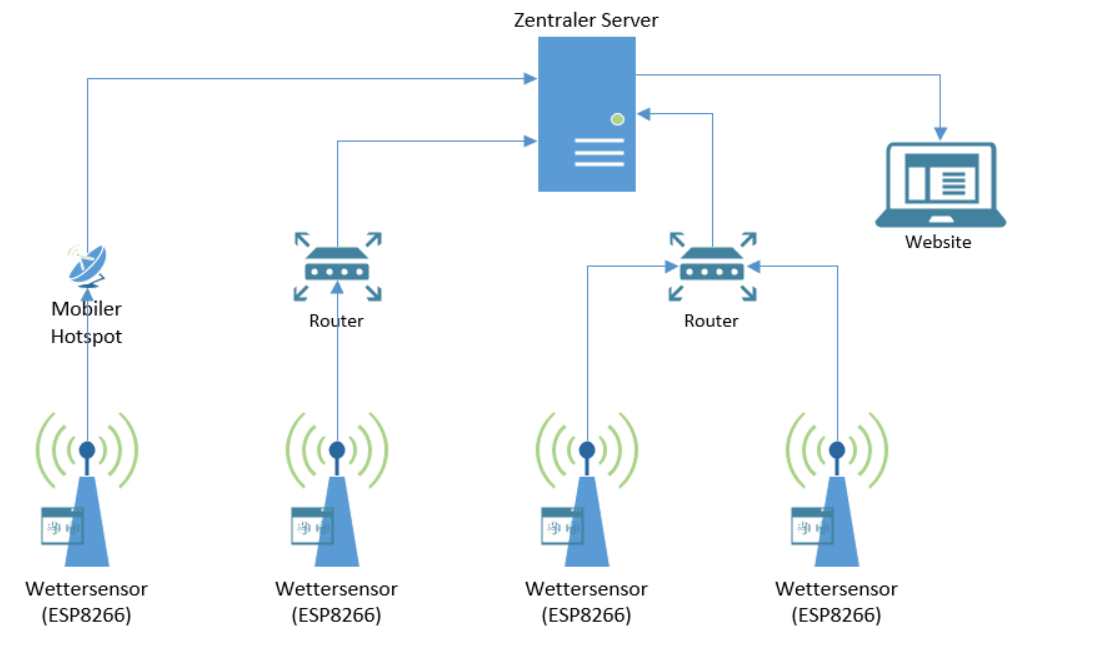
\includegraphics[width=0.7\linewidth]{img/projektkomponenten}
    \caption[Komponenten des Gesamtsystems]{Komponenten des Gesamtsystems (eigene Darstellung)}
    \label{fig:projektkomponenten}
\end{figure}
\\
In \autoref{fig:projektkomponenten} ist ein möglicher Aufbau der Projektkomponenten gemäß den Projektanforderungen\footnote{\cite{Wortmann.2020}} dargestellt.

\subsection{Mikrocontroller}
Wie in \autoref{ESP} beschrieben, kommt im Projekt ein ESP8266 Mikrocontroller zum Einsatz. Auf dem Mikrocontroller erfolgt die Erfassung der Messdaten mit einem BME280-Sensor und der Versand an das Backend.
Bei der Auswahl der Libraries wurde hierbei beachtet, möglichst auf den Anwendungsfall spezifische Libraries zu wählen um die Auslastung des Mikrocontrollers zu minimieren.
Ein geringer Energieverbrauch wird in der Programmierung besonders beachtet. Dadurch ist die Funktionalität auf das wesentliche beschränkt während trotzdem eine zuverlässige Funktionsweise gewährleistet wird. Wenn der Mikrocontroller keine Verbindung zum angegebenen WLAN-Netzwerk herstellen kann oder der Server nicht erreichbar ist, werden die Daten gecached und versandt, sobald eine Verbindung hergestellt werden kann.\\
Der Mikrocontroller wird in der Arduino IDE in C++ programmiert.

\subsection{Zentraler Server}%TODO auf frech an dieser Stelle Zentraler Server ~ Backend -> für konstistente Benennung sorgen am Ende
Auf dem zentralen Server wird das Backend des Projekts bereitgestellt. Das Backend ist in JavaScript geschrieben und verwendet eine SQLite-Datenbank für die Speicherung der Daten. Für die Kommunikation zu den Sensoren und dem Frontend ist eine REST-API vorhanden, die in \autoref{Schnittstellen} näher erläutert wird.\\
Das Projekt nutzt node.js Version 14.4 und SQLite-Version 3.\\
Sowohl das Backend als auch das Frontend sind für das Deployment in Docker vorgesehen. Hierbei ist eine örtliche Trennung möglich, das Frontend kann auf jeden Server zugreifen, der die API dieses Projekts bereitstellt.

\subsection{Website}
Die Website basiert ebenfalls auf JavaScript für die Logik. Aufgrund des Projektaufbaus ist es wie oben genannt möglich, das Hosting von Backend und Frontend zu trennen.\\
Für die Bereitstellung des Frontends kommen einige Node-Libraries zum Einsatz. Die Darstellung der Messdaten auf der Website erfolgt mit \enquote{Chart.js}\footnote{\cite{chartjs.2020}}. Die Auswahl eines Zeitraums für die Darstellung eines Intervalls ist mit der Library \enquote{daterangepicker}\footnote{\cite{daterangepicker.2020}} umgesetzt. Für die Konnektivität mit dem Backend nutzen wir \enquote{Express}\footnote{\cite{express.2020}}, dadurch wird das Handling der Serving der Frontend-Ressourcen deutlich vereinfacht. Zusätzlich wurde für das Projekt \enquote{Browserify}\footnote{\cite{browserify.2020}} verwendet, um zu verhindern, dass mehrere Dateien im Frontend geserved werden müssen, indem die einzelnen Dateien zu je einer Datei für die Haupt- und Adminseite zusammengefasst werden.
Die HTML- und CSS-Komponenten der Website sind mit Bootstrap 4 erstellt worden. Auf die Gestaltung wird in \autoref{GUI-Konzept} näher eingegangen.

    \section{ER-Diagramm}
In diesem Kapitel wird die Datenbankstruktur des Projekts dargestellt.\\
\begin{figure}[h]
    \centering
    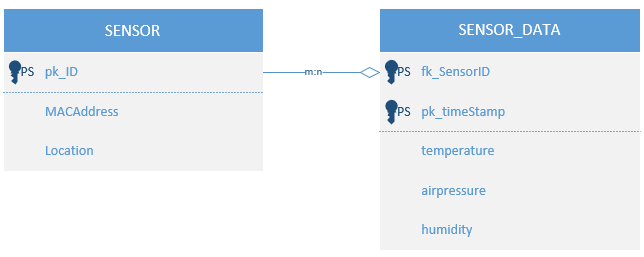
\includegraphics[width=1\linewidth]{img/erd}
    \caption[ER-Diagramm des Projekts]{ER-Diagramm des Projekts (eigene Darstellung)}
    \label{fig:erd}
\end{figure}

In \autoref{fig:erd} ist das ER-Diagramm des Projekts dargestellt. Die Datenbankstruktur ist bewusst simpel aber erweiterbar gehalten.
\subsection*{SENSOR}
Die Tabelle Sensor beinhaltet alle Informationen über die Sensoren des Systems.
Neben einer vom System vergebenen ID sind Informationen über die MAC-Adresse und den Standort enthalten.
Die MAC-Adresse wird bei jeder Request vom System zur Identifikation mitgeschickt und dient im Backend der Zuordnung von Messwerten zu Sensoren. Die MAC-Adresse wird als String gespeichert, es findet jedoch im Backend eine Überprüfung statt, die sicherstellt dass keine fehlerhafte Formatierung möglich ist.
Die Spalte \enquote{Location} ermöglicht die Zuordnung eines Standorts zu einer Messstation. Dieser Wert kann im Frontend nur durch den Administrator festgelegt werden, weshalb hier keine besondere Datenvalidierung notwendig ist und die Speicherung als String die größtmögliche Flexibilität bietet.
\subsection*{SENSOR\_DATA}
In dieser Tabelle werden die einzelnen Datensätze gespeichert. Ein Datensatz besteht standardmäßig aus einem Zeitstempel, und je einem Messwert für Temperatur, Luftdruck und -Feuchtigkeit. Die Einzigartigkeit eines Datensatzes wird durch die Vereinigung der Sensor-ID und des Zeitstempels sichergestellt. Der Sensor überträgt die oben genannten Daten zusätzlich zu seiner eigenen MAC-Adresse. Im Backend wird vor dem Speichern des Messwerts anhand der MAC-Adresse die Sensor-ID ermittelt (wenn der Sensor bereits bekannt ist) oder neu vergeben und dem Request hinzugefügt, mit dem die Daten dann in die Datenbank eingefügt werden. Zeitstempel und die drei Messwerte sind hierbei numerisch gewählt, wobei integer als Datentyp ausreichend ist, um die möglichen Zeitstempel abzudecken und beispielsweise float genügt, um die möglichen Messwerte mit Komma zu speichern. Im Backend erfolgt eine Validierung der Daten, die verhindert dass verfälschte Messwerte oder Zeitstempel (zum Beispiel in Folge eines Messfehlers) in die Datenbank geraten.\\

    %%!TEX root = ../Thesis.tex


\section{Projekt-Architektur}\label{Projekt-Architektur}
Die Ordnerstruktur des Projekts ist in \autoref{fig:dir_struc_root} zu sehen.
Die Strukturen für das Frontend, Backend sowie den NodeMCU Code sind im Anhang \ref{anh:Projekt-Architektur} zu finden.

\begin{figure}[H]
    \centering
    \begin{minipage}[t]{1\textwidth}
        \caption{Root-Ordnerstruktur}
        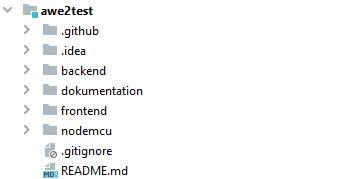
\includegraphics[width=0.5\textwidth]{img/dir_struc_root.png}\\
        \source{Eigene Darstellung}
        \label{fig:dir_struc_root}
    \end{minipage}
\end{figure}

Die Quelltexte der drei Komponenten NodeMCU, Backend und Frontend sind voneinander getrennt, werden aber als ein Gesamtprojekt ausgeliefert.

\subsection{Frontend}
Die Struktur des Frontend-Quellcodes ist eine Mischung aus klassicher Web- und Nodejs- Projektstruktur.
In dem Ordner \textit{resources} sind Ressourcen zu finden, welche der Webserver den Clients bereitstellt.
Diese sind in \textit{css}, \textit{img} und \textit{js} gegliedert.
Verwendete Libraries, wie z.B. \textit{sir.js} befinden sich in eigenen Unterordnern, während der eigenentwickelte
Quellcode sich direkt in den Ordnern befindet.

Im Root-Ordner des Frontends befinden sich, für die Komponente, globale Dateien, wie z.B. das Buildscript für Docker,
die \textit{package.json} für Node.js und die \textit{.eslintrc.json} zur Konfiguration des JavaScript-Linters.

\subsection{Backend}
Die Struktur das Backend-Quellcodes orientiert sich an der üblichen Struktur für Node.js Projekte, ist jedoch
absichtlich simpel und flach, anstatt tief hierarchisch, gestaltet.
Dies ermöglicht bei der kleinen Größe der Anwendung eine effizientere Navigation durch die Dateien.
In dem Unterordner \textit{src} befinden die Quelltexte des Backends, in \textit{test} die Quelltextdatei testMain.js
sowie die testData.js, welche nur zum Generieren von Testdaten verwendet wird.
\subsection{NodeMCU}
In dieser Komponente befindet sich im Unterordner \textit{src/nocemcu} die aktuell einzige Quelltextdatei für den NodeMCU.
Im Ordner \textit{ress} befindet sich zusätzlich eine Tabelle des Wirings von dem NodeMCU und dem BME280-Sensor.







    %%!TEX root = ../Thesis.tex


\section{Abläufe}\label{Ablaeufe}
In diesem Kapitel werden die Abläufe der jeweiligen Anwendungen (vereinfacht) dargestellt. Für die Komponenten
Backend und NodeMCU wurde jeweils ein UML-Diagramm erstellt. Für das Frontend wurde darauf verzichtet, da bereits
ein Use-Case-Diagramm besteht und der technische Aufbau sehr überschaubar ist. Die UML-Diagramme befinden sich in Anhang
\ref{anh:ablaeufe}.

\subsection{Backend}
In \autoref{fig:backend_activity} ist ein Aktivitätendiagramm zu sehen. In diesem ist der simple Aufbau des Backends
zu erkennen. Hierbei handelt es sich um einen klassischen Webserver, der Requests empfängt und verarbeitet.

\subsection{NodeMCU}
Das Zustandsdiagramm ist in \autoref{fig:zust_diag_nodemcu_setup}, \autoref{fig:zust_diag_nodemcu_loop} und
\autoref{fig:zust_diag_nodemcu_send} zu sehen. Es wurde zu Gunsten der Übersichtlichkeit in drei Teile aufgeteilt.
Nach dem Boot wird in die setup-Funktion gesprungen.
In dieser wird nach einem BME280 Sensor gesucht.
Insofern einer gefunden wurde, wird die WLAN-Verbindung aufgebaut.
Anschließend wird die loop-Funktion endlos in einer Schleife aufgerufen.
Diese beginnt mit dem Auslesen der Sensordaten, welche in eine Liste gespeichert werden.
Wenn die Liste voll ist, wird das erste Element zuvor entfernt.
Nach Prüfung, ob die WLAN-Verbindung vorhanden ist, wird die sendCachedData-Funktion aufgerufen.
In dieser wird über alle Listenelemente iteriert.
In jeder Iteration wird eine HTTP-Verbindung zum Backend aufgebaut.
Anschließend wird ein eventuell inkorrekter Timestamp (mit Wert = 0) korrigiert.
Danach wird der JSON-String für den HTTP-Body aus den Daten erstellt.
Nach anschließendem Versenden wird der HTTP-Code ausgewertet.
Bei einem erwarteten Wert wird das Element aus der Liste entfernt.
Zuletzt wird die HTTP-Verbindung geschlossen und in die nächste Iteration gegangen.
Mit dem Ende der Iterationen endet die Funktion, womit in die loop-Funktion zurückgekehrt wird.
Nach Warten einer Verzögerung wird diese erneut (endlos) aufgerufen.


    %!TEX root = ../Thesis.tex
\section{Schnittstellen}\label{Schnittstellen}
Das Backend unserer Anwendung verfügt über eine REST-API.
Diese wird zur Kommunikation des Backends mit den jeweiligen Wettersensoren, sowie zur Kommunikation des Frontends mit dem Backend verwendet.

\subsection*{Schnittstellenbeschreibung REST-API}\label{schnittstellen:rest}
Die Schnittstelle stellt folgende Services bereit:

\begin{itemize}
    \item \textsl{HTTP-Methode}: GET
    \subitem \textsl{Relativer Pfad}: \textbf{/weatherData}
    \subitem \textsl{Antwort}: JSON-Object mit zwei Arrays.
    Das Erste beinhaltet alle Sensoren, das Zweite alle verfügbaren Sensordaten.\footnote{Für beinhaltete Datentypen siehe \cref{er-diagramm}}
    \subitem \textsl{Beispielantwort}: siehe Anhang \ref{Anhang:Schnittstellen}
\end{itemize}

\begin{itemize}
    \item \textsl{HTTP-Methode}: GET
    \subitem \textsl{Relativer Pfad}: \textbf{/sensorData/id/:SENSOR\_ID}
    \subitem \textsl{Antwort}: JSON-Object mit Wetterdaten für gewählten Sensor
    \subitem \textsl{Parameter}: \begin{itemize}
                                     \item URL-Encoded: \textit{ID} - ID des gewünschten Sensor
                                     \item (optional) Query:    \textit{timerange\_start} - Mindestzeitstempel der Sensordaten.
                                     \item (optional) Query:    \textit{timerange\_end} - Höchstzeitstempel der Sensordaten.
                                     \item (optional) Query: \textit{granularity} - Menge der zurückzugebenden Datenpunkte
    \end{itemize}
    \subitem \textsl{Beispielantwort}: siehe Anhang \ref{Anhang:Schnittstellen}
\end{itemize}

\begin{itemize}
    \item \textsl{HTTP-Methode}: GET
    \subitem \textsl{Relativer Pfad}: \textbf{/sensors}
    \subitem \textsl{Antwort}: JSON-Object welches alle Sensoren beinhaltet.
    \subitem \textsl{Beispielantwort}: siehe Anhang \ref{Anhang:Schnittstellen}
\end{itemize}

\begin{itemize}
    \item \textsl{HTTP-Methode}: GET
    \subitem \textsl{Relativer Pfad}: \textbf{/sensor/id/:SENSOR\_ID}
    \subitem \textsl{Antwort}: JSON-Object welches die Informationen über einen ausgewählten Sensor beinhaltet.
    \subitem \textsl{Parameter}: \begin{itemize}
                                     \item URL-Encoded: \textit{ID} - ID des gewünschten Sensor
    \end{itemize}
    \subitem \textsl{Beispielantwort}: siehe Anhang \ref{Anhang:Schnittstellen}
\end{itemize}

\begin{itemize}
    \item \textsl{HTTP-Methode}: POST
    \subitem \textsl{Relativer Pfad}: \textbf{/weatherData/}
    \subitem \textsl{Inhalt}: JSON-Object welches Sensordaten beinhaltet.\footnote{Für beinhaltete Daten siehe \cref{er-diagramm}}
    \subitem \textsl{Antwort bei Erfolg}: HTTP-Status 200, String der erfolgreiche Speicherung bestätigt
    \subitem \textsl{Antwort bei Fehlern}:\begin{itemize}
                                              \item \textit{Duplizierter Inhalt}: HTTP-Status 400, Fehlermeldungen und Errors
                                              \item \textit{Fehler beim Parsen des Bodies}: HTTP-Status 400, Fehlermeldungen und Errors
    \end{itemize}
\end{itemize}

\begin{itemize}
    \item \textsl{HTTP-Methode}: POST
    \subitem \textsl{Relativer Pfad}: \textbf{/updateSensorLocation/}
    \subitem \textsl{Inhalt}: JSON-Object welches aktualisierten Ort für über ID identifizierten Sensor beinhaltet.
    \subitem \textsl{Absicherung}: Dieser Endpoint kann nur durch mitsenden eines API-Tokens genutzt werden.\footnote{Dieser steht nur dem Admin zur Verfügung und ist genauer unter \cref{Security} spezifiziert.}
    \subitem \textsl{Antwort bei Erfolg}: HTTP-Status 200, String der erfolgreiche Speicherung bestätigt
    \subitem \textsl{Antwort bei Fehlern}:\begin{itemize}
                                              \item \textit{Fehler beim Parsen des Bodies}: HTTP-Status 400, Fehlermeldungen und Errors
    \end{itemize}
\end{itemize}




    %!TEX root = ../Thesis.tex
\section{Security}\label{Security}
Im folgenden werden getroffene (Design)-Entscheidungen in Bezug auf die Sicherheit unserer Anwendung erläutert.
Dabei werden besonders relevante Stellen hervorgehoben und erklärt.
Die Erläuterung ist aufgeteilt in die Bestandteile unserer Anwendung.

\subsection{ESP8266}

%- WLAN Hardcoded Designentscheidung -> vernunft -> gezielte Platzierung ESP
Die \textit{Wlan Zugangsdaten} werden beim flashen unserer Anwendung auf den ESP übertragen und sind ab diesem Punkt fest / \enquote{hardcoded}.
Diese Entscheidung wurde getroffen unter der Abwegung, dass die ESPs, und damit die Wettersensoren, einen festen Standort besitzen.\footnote{Darüber hinaus ist anzumerken, dass sowieso die letzte WLAN-Verbindung im ESP gehalten wird, auch wenn neuer Code geflasht wird. Somit dürfen die Geräte nicht durch Unbefugte benutzt werden.}
Dieser wird wie bereits erläutert im Admininterface der jeweiligen MAC-Adresse des Gerätes zugeordnet.
Hierdurch bedingt war eine mögliche dynamische Festlegung der Zugangsdaten für uns nicht verhältnismäßig.
Insbesondere da ohne WLAN-Verbindung keine Kommunikation mit dem Gerät erfolgen kann.\\
%- keine Absicherung Rest Calls -> Leistung / Aufwand / Nutzen
Der zweite relevante Punkt ist die \textit{Absicherung von REST-Calls}.
Wir haben uns im Hinblick auf die geringe Leistung der ESPs gegen eine weitere Absicherung der REST-Calls entschieden.
Um aufgrund der Corona-Situation eine Zusammenarbeit zu ermöglichen wurde die Anwendung öffentlich erreichbar gemacht.
Grundsätzlich ist dies aber kein notwendigerweise geplanter Einsatzzweck.
Diese Entscheidung wird im folgenden Absatz weiter erläutert.

\subsection{Backend}

%- keine Absicherung anderer Endpoints -> interne und keine öffentliche Nutzung vorgesehen
Durch die Ausrichtung auf eine interne und nicht öffentliche Nutzung (beispielhaft in einem internen Unternehmensnetzwerk) haben wir entschieden, dass eine grundlegende Absicherung des \textit{Sensordaten Endpoints} ausreichend ist.
Diese besteht bei uns konkret in der Prüfung der empfangenen Sensordaten (Siehe \cref{schnittstellen:rest}), hier werden die Werte auf Korrektheit im Bezug auf Datentypen, sowie insbesondere sinnvolle Werte (z.B. Zeitstempel nicht vor Veröffentlichungsdatum oder Temperaturen außerhalb von festgelegten Grenzwerten) geprüft.
Des weiteren werden die Daten vor dem einfügen in die Datenbank von uns parametrisiert um SQL-Injections zu verhindern.\\
%- Absicherung Endpoint Ort -> API-Token -> Admins vorbehalten
Die Nutzung des \textit{Sensorstandort Endpoint} ist dem Administrator vorbehalten.
Deswegen ist zur erfolgreichen Änderung des Standorts ein \enquote{API-Token} notwendig.
Dieser wird bei Änderungen des Standorts im Frontend mitgesendet.
Diese Absicherung ist grundlegend da nur Administratoren diesen \enquote{API-Token} durch einen erfolgreichen Login erlangen können.
Nach Abwegung des möglichen Schaden gegenüber den Kosten der Implementierung haben wir von einer weiteren Absicherung abgesehen.\\
%- Logging verwendet Siehe Anhang \ref{anhang:logdaten}
Darüber hinaus nutzt unsere Anwendung \textit{Logging}.
Eingehende Anfragen und insbesondere Fehler werden durch das Node-Modul \texttt{rotating-file-stream} geloggt.
Dieses ist so konfiguriert, dass Events mit Zeitstempel und Dringlichkeit (beispielhaft \enquote{INFO} oder \enquote{ERROR})in die Konsole geloggt werden.
Beim auftreten von Errors werden die fehlerhaften Requests in Gänze geloggt, da dies notwendig ist um die Quelle dieser nachzuvollziehen.
Darüber hinaus werden alle Log-Nachrichten in einer Datei gespeichert.
Diese ist auf 10 Megabyte Größe begrenzt und wird täglich gewechselt.
Alte Dateien werden komprimiert gespeichert.
Auszüge hiervon finden sich im Anhang \ref{anhang:logdaten}.

\subsection{Frontend}

%- Logging verwendet Siehe Anhang \ref{anhang:logdaten}
Das Frontend-Modul verwendet die Selbe \textit{Logging Konfiguration} wie das Backend.
Auszüge hiervon finden sich im Anhang \ref{anhang:logdaten}.\\
%- Basic Auth Login Admin Interface -> Ausreichend weil nur Ort veränderbar
Erwähnenswert ist hier insbesondere das \textit{Admin-Interface}.
Der Zugang hierzu kann erst nach erfolgreichem Login mit Hilfe von Basic-Authentication erfolgen.
Da im Admin-Interface nur die Funktionalität der Festlegung des Sensorstandortes verfügbar ist, ist diese Lösung die effektivste und sinnvollste zur Gewährleistung der Sicherheit.

\subsection{Github}

%- Dependencies Check auf CVE / Updates -> Notification
Im Zuge der Versionsverwaltung unseres Projektes werden alle Module, wie von uns explizit konfiguriert, \textit{automatisiert auf Sicherheitslücken} überprüft.
Sollte durch Github eine Sicherheitslücke in Libraries oder Code gefunden werden, so werden wir als Entwickler benachrichtigt.
Mit dieser Maßnahme lassen sich potentielle Sicherheitslücken schnell und automatisiert finden und einfach beheben.\\

\subsection{Deployment}

%- Live Deployment vorgesehen hinter zusätzlichem Proxy welcher Traffic filtert und überwacht, sowie ggf. Fail2Ban o.ä. bereitstellt.
Das Deployment unserer Anwendung ist mit Hilfe von Docker realisiert.
Wie während der Entwicklung umgesetzt, ist ein etwaiges Live-Deployment im besten Fall hinter einem \textit{zusätzlichen Reverse-Proxy-Server} zu realisieren\footnote{Hierzu wurde während der Entwicklung ein \cite{swag} Docker Container genutzt, alternativ kann \cite{traefik} als Docker Container genutzt werden}.
Dadurch ergibt sich eine zusätzliche Instanz welche zum Schutz der Anwendung beiträgt. Mit Hilfe des Reverse-Proxy-Servers können Anfragen an Frontend sowie Backend überwacht und gefiltert werden.
Darüber hinaus lassen sich IP-Adressen böswilliger Anfragen sperren.
Dies lässt sich mit einem System wie \cite{Fail2Ban} realisieren.\footnote{Dieses ist in \cite{swag} bereits inkludiert}\\
%- Deployment automatisierbar einbinden von Dockerfile auf Server -> automatisches bauen v. Image mit neuestem Stand
Ebenso sollte auf dem Deployment-Server im Zuge der Dockerverwaltung ein \textit{automatisches Update der Container} konfiguriert werden, wie während der Entwicklung geschehen.
Hierbei werden mit Hilfe der Dockerfiles die Images regelmäßig neu gebaut, um Abhängigkeiten auf dem neuesten Stand zu halten.
Anschliessend werden die verwendeten Images der Container ausgetauscht.
Zum automatisierten Bau der Images, sollte ein \enquote{Cron-Job} genutzt werden.
Um die Nutzung der neuesten Images zu gewährleisten bietet sich \cite{watchtower}, ebenfalls als Docker Container, an.


    %!TEX root = ../Thesis.tex


\section{Tests}\label{Tests}

\subsection{Automatische Tests}
Für die relevantesten Funktionen der Anwendung wurden Unit-Tests geschrieben.
Im Backend sowie Frontend wurden die Frameworks Chai\footnote{\cite{chai}} und Mocha\footnote{\cite{mocha}} verwendet.
Chai ist eine Assertion Library, während Mocha ein komplettes Test-Framework ist.
Die Struktur der Tests wird somit durch Mocha vorgebenen.
Durch Chai werden lediglich die Assertions evaluiert.
Die Testklassen heißen jeweils testMain.js und befinden sich in den src/test Ordnern des Front- und Backends.
\subsubsection*{Testabdeckung}
Die erreichte Testabdeckung ist in \autoref{fig:tc_frontend} und \autoref{fig:tc_backend} zu sehen.
\begin{figure}[H]
    \centering
    \begin{minipage}[t]{1\textwidth}
        \caption{Testabdeckung Frontend}
        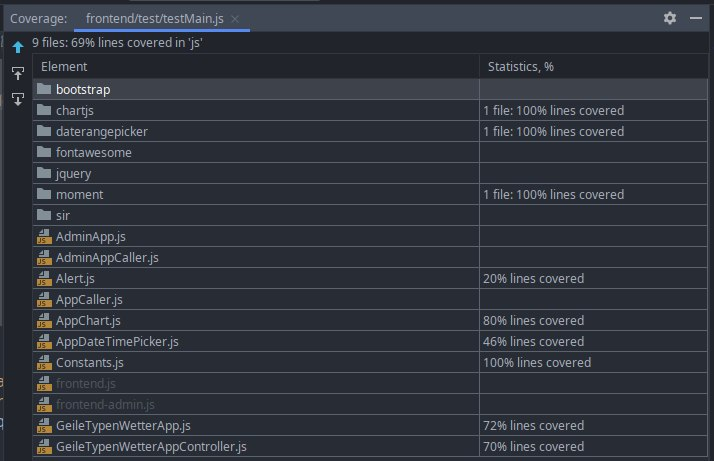
\includegraphics[width=1\textwidth]{img/tc_frontend2.png}\\
        \source{Eigene Darstellung}
        \label{fig:tc_frontend}
    \end{minipage}
\end{figure}
\begin{figure}[H]
    \centering
    \begin{minipage}[t]{1\textwidth}
        \caption{Testabdeckung Backend}
        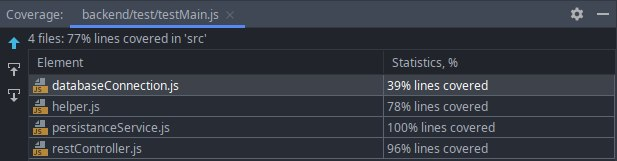
\includegraphics[width=1\textwidth]{img/tc_backend2.png}\\
        \source{Eigene Darstellung}
        \label{fig:tc_backend}
    \end{minipage}
\end{figure}
\subsection{Manuelle Klicktests}
Es wurden manuelle Tests der Benutzoberfläche ausgeführt, um etwaige Fehler dort zu entdecken.
Diese wurden dokumentiert.
\subsubsection*{Inhalte}
Bei der Durchführung der manuellen Klicktests sollen folgende Inhalte dokumentiert werden:
\begin{itemize}
    \item Git Commit Hash (Anwendungsversion)
    \item Git Branch
    \item Verwendetes Betriebssystem
    \item Verwendeter Browser inkl. Build
    \item Screenshots bei Darstellungsfehlern
    \item Bildschirmauflösung, insbesonders bei mobiler Ansicht
\end{itemize}
Die Testdurchführung befindet sich in Anhang \ref{anh:testplan}.

    \section{Anwendungsfälle}
In diesem Kapitel wird das Use Case Diagramm dargestellt, welches die Anwendungsfälle der Website darstellt.
Da das Backend und der Mikrocontroller keine direkte Interaktion mit dem User ermöglichen, werden sie hier nicht erfasst.\\
\begin{figure}[h]
    \centering
    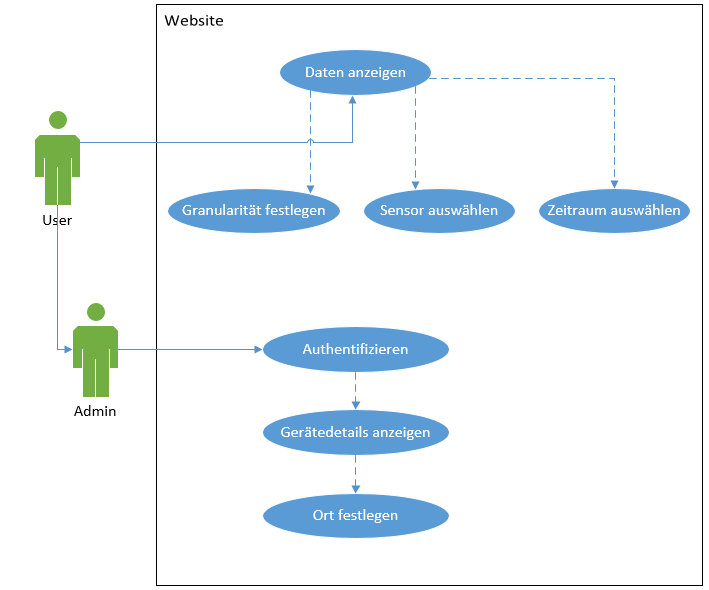
\includegraphics[width=0.7\linewidth]{img/usecase}
    \caption[Use Case Diagramm des Projekts]{Use Case Diagramm des Projekts (eigene Darstellung)}
    \label{fig:usecase}
\end{figure}

Der User hat auf der Website einen primären Anwendungsfall mit einigen Erweiterungen.
Neben der Anzeige der Daten kann der User die Granularität festlegen, also ändern wie viele Datenpunkte im Diagramm angezeigt werden.
Außerdem kann ein anderer Sensor aus dem Dropdown ausgewählt werden, um dessen Messwerte darzustellen.
%TODO sog. Daterangepicker erklären
Über den sogenannten \enquote{Daterangepicker} kann der Zeitraum festgelegt werden, in dem die Messdaten angezeigt werden. \\
Der Administrator hat neben den Anwendungsfällen des Users zusätzlich die Möglichkeit sich mit Nutzernamen und Passwort zu authentifizieren um das Administrator-Interface anzuzeigen.
Dort sind Gerätedetails aufgeführt und der Administrator kann den Standort des Sensors festlegen.

    %!TEX root = ../Thesis.tex


\section{GUI-Konzept}\label{GUI-Konzept}

Dieses GUI-Konzept entspricht dem Stand vor dem Beginn der Entwicklung unseres Prototypen.
Hilfreich war hierbei, dass zu diesem Zeitpunkt bereits die zu nutzenden Technologien festgelegt waren.
Für das Konzept, abgebildet in \cref{fig:gui-konzept}, wurde \enquote{Bootstrap 4}\footnote{\cite{bootstrap}} genutzt.
Hierdurch sind alle Buttons sowie UI-Elemente grundlegend einheitlich.
Dies findet sich insbesondere in der Navigationsleiste sowie den Buttons und Input-Feldern wieder.
Die Sprache des Frontends ist Englisch, da dies eine Internationalität ermöglicht.
Innerhalb der Navigationsleiste findet sich zur linken der Name unserer Anwendung sowie unser Logo.
Letzteres stellt stilisiert einen Regenschirm mit Funkverbindung da.
Eine humoristische Anspielung auf den Einsatzzweck unserer Anwendung.

\begin{figure}[h!!]
    \centering
    \begin{minipage}[t]{1\textwidth}
        \caption{GUI-Konzept}
        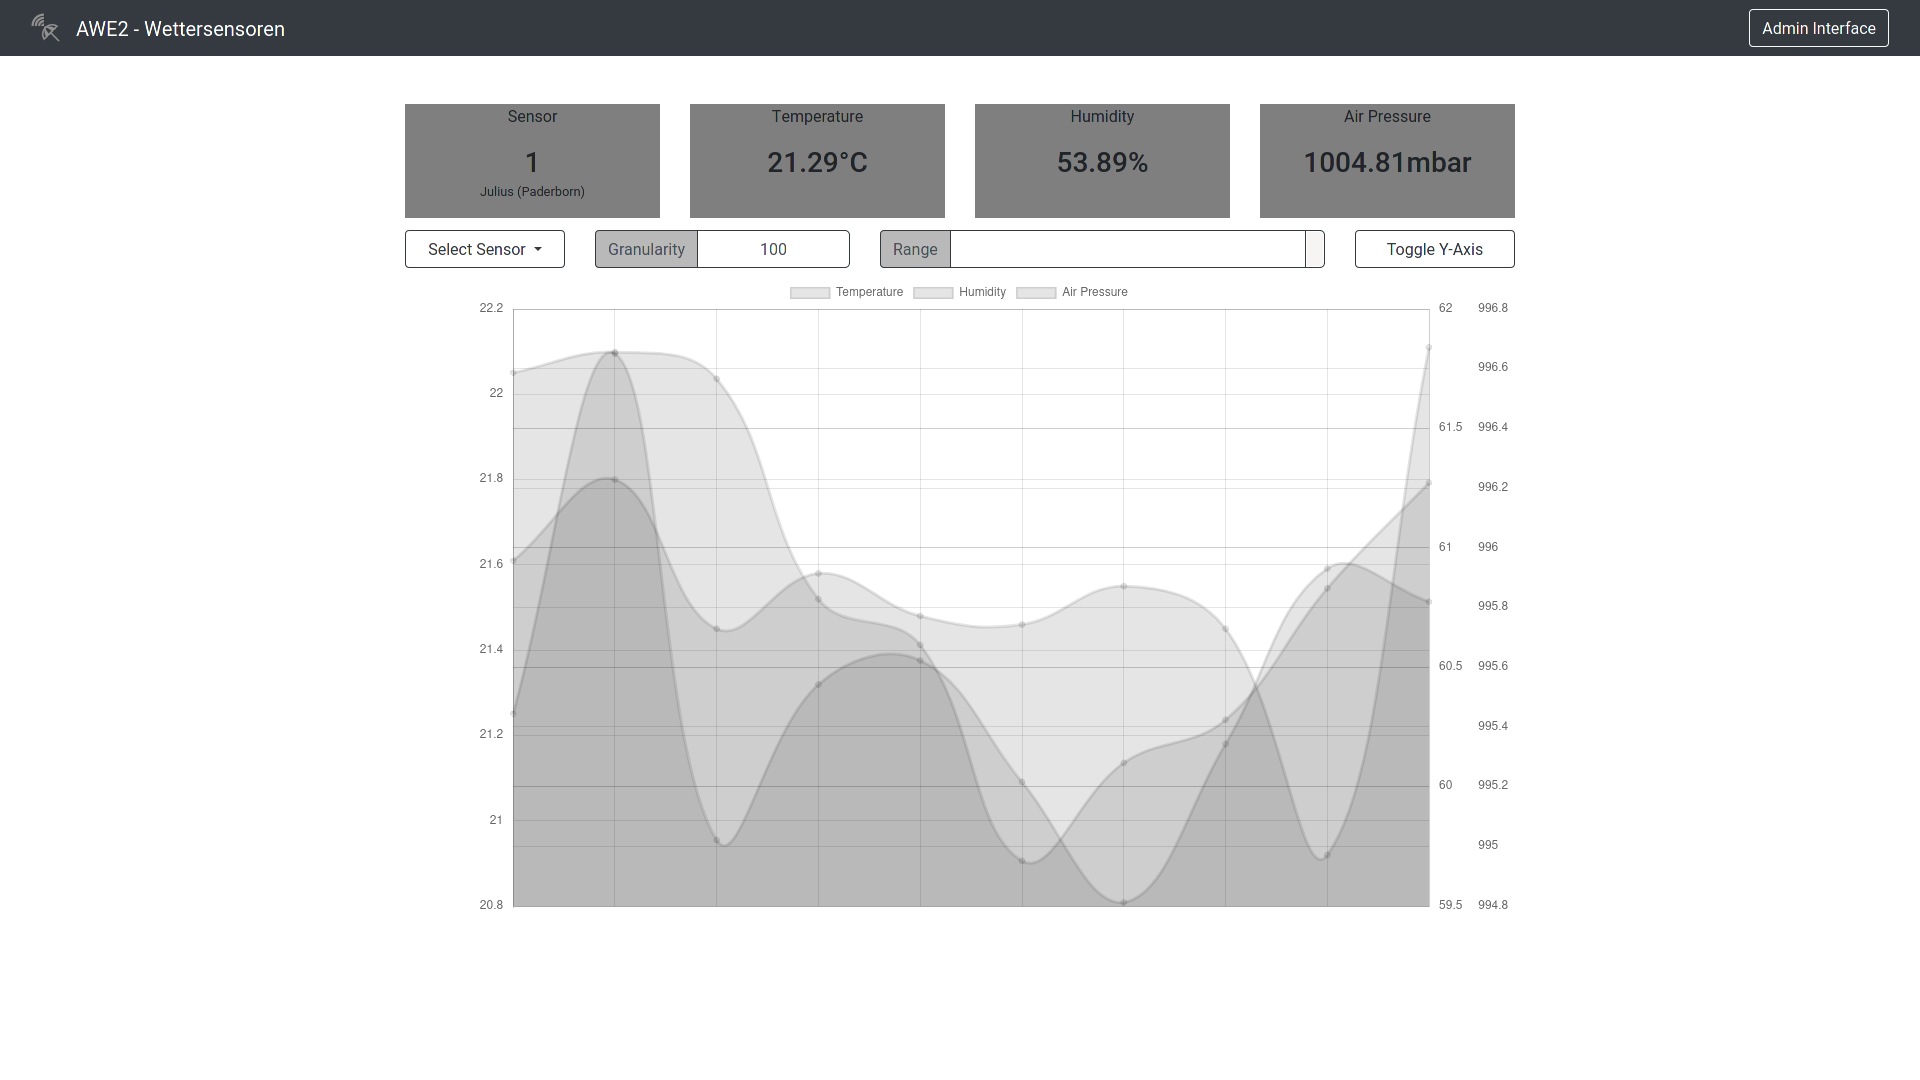
\includegraphics[width=1\textwidth]{img/gui-konzept.png}\\
        \source{Eigene Darstellung}
        \label{fig:gui-konzept}
    \end{minipage}
\end{figure}

Ziel unseres Konzeptes war es eine konsistente, einheitliche und leicht verständliche Benutzeroberfläche zu generieren.
Der Fokus unserer Anwendung ist die Darstellung und Auswertung von Wettersensoren. Unter diesen Aspekten wurde die Oberfläche entwickelt.
Informationen sind zentral gehalten, direkt ersichtlich sind vier Blöcke mittig auf dem Bildschirm platziert.
Durch diese ist einerseits der zurzeit ausgewählte Sensor und andererseits alle drei aktuellen Sensorwerte im direkten Fokus des Anwenders.
Alle Einstellungsmöglichkeiten sind innerhalb einer darunterliegenden Reihe platziert.
Die Auswahl des darzustellenden Sensors erfolgt direkt unter der Ansicht des Aktuellen, auch hierdurch wird die Bedienung klar und für den Anwender einfach gehalten.
Daneben finden sich alle weiteren Eingabemöglichkeiten für Parameter der Graphen.
Das Hauptelement in Form der Graphen wird durch \enquote{chart.js}\footnote{\cite{chartjs.2020}} bereitgestellt.
Hier haben wir uns entschieden alle Sensorverläufe innerhalb eines Graphen zu plotten um diese zentral und sichtbar zu halten.
Hier ist insbesondere anzumerken, dass Achsenbeschriftungen sowie Einfärbungen noch nicht vorhanden sind, da diese innerhalb des Codes durch Konfigurationen angepasst werden.

Durch die frühe Festlegung der Positionierung sowie der gesamten Oberfläche konnte sich während der Entwicklung auf die technische Implementierung konzentriert werden, da das fertige Design nur umgesetzt werden musste.
So war es im folgenden nur noch notwendig geringfügige Anpassungen vorzunehmen um der Anwendung den letzten Schliff zu geben.
Nach der Entwicklung des ersten Prototypen haben wir Dies einerseits in der Entwicklung eines einheitlichen Farbenkonzeptes umgesetzt.
Die in \cref{fig:farbmuster} abgebildeten Farben basieren in den hellen sowie dunklen Tönen auf Bootstrap Standart-Farben.
Für die weiteren Farbtöne haben wir uns eine Pastell-Farb-Palette ausgesucht. Diese wurden im folgenden einheitlich genutzt.
Der Gelbton wurde ausschließlich für Informationen benutzt, die restlichen Farben wurden jeweils für Temperatur, Luftfeuchte und Luftdruck genutzt.
Dies findet sich innerhalb der Blockelemente in der oberen Reihe aber auch insbesondere im Chart innerhalb der Graphen wieder, wo die Farben hervorhebend eingesetzt wurden.
Anderseits wurden die Informationen um passende \enquote{Font Awesome}-Icons\footnote{\cite{fontawesome}} ergänzt.
Hierdurch wird eine Orientierung auf der Oberfläche nochmals erleichtert und verbessert.
Darüber hinaus wurden die Block Elemente innerhalb der GUI um runde Kanten ergänzt, hierdurch bekam die Anwendung eine modernere zeitgemäßere Oberfläche. Die insbesondere konsistenter und passender zu den in Bootstrap vorhandenen Buttons ist.
\begin{figure}[h!!]
    \centering
    \begin{minipage}[t]{1\textwidth}
        \caption{Farben-Konzept}
        \includegraphics[width=0.5\textwidth]{img/Farbmuster.png}\\
        \source{Eigene Darstellung}
        \label{fig:farbmuster}
    \end{minipage}
\end{figure}

Die fertige GUI findet sich im Anhang \ref{gui-fertig}.
Weitere GUI-Elemente werden hier ebenfalls beschrieben.
Dazu gehören die Datumsauswahl in Anhang \ref{datumsauswahl}, das Admininterface im Anhang \ref{admininterface}, sowie die Informationsmeldungen im Anhang \ref{popup}.
Als netter Nebeneffekt ergab sich durch die Nutzung von Bootstrap, mit Hilfe geringer Anpassungen, eine nahezu vollständige Kompatibilität zu Mobilgeräten, auch wenn Diese nicht gefordert war.






    \section{Projektplanung}
Für das Projekt wurden zahlreiche Projektmanagementtools eingesetzt.
Diese werden in diesem Kapitel erläutert.

\subsection{Verwendete Tools und Methodik}
Für das Projektmanagement wurde Trello genutzt.
Trello ist die führende Online-Plattform für Kanban\footnote{vgl. \cite{atlassian}}.
Aufgrund der Struktur der Gruppe und des Projektumfangs bietet sich Kanban als Projektmanangementmethode an.
Die Features werden als Arbeitspakete in Karten aufgeteilt und zugewiesen.
Zusätzliche Karten werden angelegt, um organisatorische Features, Karten für Bugfixes und Randaufgaben (wie Refactoring) erweitert.
Der Vorteil von Trello und Kanban für das Projekt sind besonders aufgrund der Corona-Situation gegeben, da es auch ohne ausführliche Besprechungen ermöglicht einzusehen, welches Gruppenmitglied aktuell an welchem Arbeitspaket arbeitet und welche Arbeitspakete vor der Vervollständigung stehen.
Die drei üblichen Kanban-Bereiche \enquote{Neu}, \enquote{In Arbeit} und \enquote{Fertig} werden hierbei in Anlehnung an agile Softwareentwicklung in die folgenden Bereiche erweitert:
\begin{itemize}
    \item \textbf{Nicht im Backlog}: In diesen Bereich kann auch außerhalb von einem Meeting jedes Gruppenmitglied Karten hinzufügen, die für sinnvoll erachtet werden. Karten in diesem Bereich werden beim folgenden Meeting diskutiert und gegebenenfalls ins Backlog geschoben.
    \item \textbf{Backlog}: Dieser Bereich beinhaltet alle Karten, die zur Bearbeitung anstehen. Karten in diesem Bereich werden in der Regel bei einem Meeting einem oder mehreren Gruppenmitgliedern zugewiesen.
    \item \textbf{In Arbeit}: In diesen Bereich werden Karten geschoben, die aktuell bearbeitet werden.
    \item \textbf{In Prüfung}: Nach der Fertigstellung einer Karte werden die entwickelten Features vom gesamten Team im nächsten Meeting überprüft. Dadurch stellen wir eine hohe Code-Qualität sicher und können bei Bedarf Karten für Bugfixes oder Refactoring in das Backlog schieben. Arbeitspakete bleiben hier bis zur Fertigstellung aller verwandten Bugfixes.
    \item \textbf{Fertig}: Nach der erfolgreichen Review werden alle fertiggestellten und auf ihre korrekte Funktionsweise überprüften Arbeitspakete in diesen Bereich geschoben.
\end{itemize}
Ein Screenshot der gesamten Arbeitspakete des Projekts findet sich in der Abgabe im Ordner \textit{dokumentation/nachweis\_arbeitspakete\_trello\_screenshots}\footnote{Die Zuordnung der Arbeitspakete wird anhand der Symbole unten rechts in den Karten ersichtlich: Das hellblaue Symbol steht für Philipp Röring, das dunkelblaue Symbol für Jonathan Brockhausen und das schwarze für Julius Figge.}.

\subsection{Projektmanagement}
Durch diese Struktur wurde sich explizit auch für an agile Entwicklung angelehnte Sprints entschieden.
Auf eine strikte Festlegung auf ein agiles Umfeld wie beispielsweise Scrum wurde jedoch bewusst verzichtet.
Der Grund hierfür ist die kurze Entwicklungsdauer im Semester und die geringe Gruppengröße.
Die Sprints waren dadurch in der Regel nur wenige Tage lang. \\
Für das Projekt wurde zunächst ein Prototyp nach dem Rapid-Prototyping-Prinzip\footnote{vgl. \cite{krypczyk.2019}} entwickelt.
Hierfür wurden die essentiellen Funktionen bereits in der ersten Woche umgesetzt, und damit eine rudimentäre Basis geschaffen, die in den folgenden Sprints um die zusätzlichen Features erweitert wurde.
In der nächsten Projektphase wurde der Code refactored und Fehler, die teilweise noch aus dem Prototyp stammten, behoben.
Durch diese Projektplanung konnte das Projekt bereits einen Monat nach Beginn für feature-complete erklärt werden.
Danach wurden nur noch später entdeckte Fehler behoben und die Dokumentation erstellt.

\subsection{Soll-Ist-Vergleich}
Die einzelnen Features, deren Einstufung und der Status sind im Anhang in \autoref{anh:sollist} aufgeführt.
Die Darstellung basiert auf \cite{Wortmann.2020} und wurde in Muss-, Kann und Bonus-Anforderungen gegliedert. Bonusanforderungen waren hierbei zunächst nicht genannt, kamen jedoch in Besprechungen als mögliche Erweiterung hinzu.
Das Projekt wurde von Anfang an so konzipiert, dass eine hohe Unabhängigkeit der einzelnen Komponenten gegeben ist.
Die Anwendung kann beliebig auf die Gegebenheiten angepasst werden, eine örtliche Trennung sind genauso möglich wie der Fernzugriff auf die Daten und die Verbindung des Sensors mit einem mobilen Hotspot.
Auch während des Betriebs können einzelne Bestandteile des Projekts bei Bedarf in den Konfigurationsdateien neu eingestellt werden.
Alle Anforderungen wurden so umgesetzt, dass auch eine Veränderung oder Erweiterung der Software im späteren Verlauf problemlos möglich ist. 

    %!TEX root = ../Thesis.tex
\section{Schlussbetrachtung}\label{Schlussbetrachtung}

\subsection{Bewertung}\label{subsec:bewertung}
%TODO siehe Projektplanung
Alle Muss-Features wurden erfolgreich implementiert.
Auch die meisten Kann-Features wurden umgesetzt. Lediglich die
Wetterprognose wurde nicht entwickelt, da sie nach weiterer Recherche aus den gewonnenen Daten zu ungenau gewesen wäre.
Alle Features wurden gemäß der Projektplanung fristgerecht fertiggestellt.
Sämtliche Deadlines konnten insbesonders durch den frühen Projektstart eingehalten werden.
Dies bezieht sich auf einzelne Teilaufgaben sowie das Gesamtprojekt.
%TODO -> rudimentäre erfahrung vlt passender oder?
Durch erste Erfahrungen der Entwickler mit JavaScript verlief der Einstieg in eine produktive Entwicklung zügig.
\\
Leider wurde das Team durch die exklusiv digitale Kommunikation - bedingt durch die anhaltende Corona-Pandemie - in der
Zusammenarbeit etwas gebremst.
Auch die - sonst übliche - hervorragende Arbeitsatmosphäre wurde dadurch verschlechtert.
\\
Die letzten Releases der Anwendung liefen über einen Zeitraum von über vier Wochen stabil auf dem Produktivsystem mit
einer Uptime von 100\%.
Darüber hinaus gab es keine Fehler in den automatischen sowie manuellen Tests des Front- und Backends.
\\
Die Qualität der erstellten Anwendung wird von den Entwicklern selbst folgendermaßen eingeschätzt (1-10 Punkte):
\begin{longtable}{|p{0.14\textwidth}|p{0.15\textwidth}|p{0.09\textwidth}|p{0.15\textwidth}|p{0.17\textwidth}|p{0.15\textwidth}|}
    \caption{Bewertung der Anwendung} \\
    \hline
    Änderbarkeit & Benutzbarkeit & Effizienz & Funktionalität & Übertragbarkeit & Zuverlässigkeit \\
    \hline
    7            & 8             & 9         & 8              & 9               & 9               \\
    \hline
\end{longtable}
Die Bewertung richtet sich nach ISO/IEC 9126. %TODO add quelle because quellen = gute note
Es folgt eine kurze Erläuterung der einzelnen Bewertungen.
Das am schlechtesten bewertete Kriterium ist die Änderbarkeit.
Diese ist auf die verwendete JavaScript Programmiersprache zurückzuführen.
Diese ist aufgrund ihrer schwachen Typisierung und inkonsistenten Implementierung anfällig für Unübersichtlichkeit bei wachsenden Anwendungen.
Sie wird jedoch für mehr als ausreichend für das Projekt in der aktuellen Größe angesehen.
Im Gegensatz dazu bietet sie zusammen mit Node.js, dem standardmäßigen Non-Blocking-IO sowie
Asynchronität eine sehr gute Effizienz für parallele Aufgaben, wie das - in diesem Fall - bereitstellen eines Webservers.
Die Fehleranfälligkeit von JavaScript wurde durch automatisierte Tests möglichst ausgeglichen, wodurch die hohe Zuverlässigkeit
entstanden ist.
Die Übertragbarkeit wird als sehr hoch eingeschätzt, da die Anwendung als Docker Image auf sämtlichen modernen
Serverumgebungen problemlos installiert werden kann.
Die Funktionalität und Benutzbarkeit entstammen unserer subjektiven Einschätzung durch manuelle Tests sowie der von
dritten Testpersonen.
\\

\subsection{Fazit}\label{subsec:fazit}%TODO add referenz soll-ist
Im Soll-ist Vergleich ist zu sehen, dass die Produktivität innerhalb des Projekts hervorragend war. Das Team bietet somit eine
gute Grundlage für weitere Zusammenarbeiten. Es wird gehofft, dass zukünftig wieder eine persönliches Zusammentreffen möglich ist,
um auch mal auf den gemeinsamen Erfolg einen Bölkstoff zischen zu können.



    %%%%%%%%%%%%%%%%%%%%%%%%%%%%%%%%%%%%%%%%%%%%%%%%%%%%%%%%%%%%%%%%%%%%%%%
    %% Anhang
    %%%%%%%%%%%%%%%%%%%%%%%%%%%%%%%%%%%%%%%%%%%%%%%%%%%%%%%%%%%%%%%%%%%%%%%

    %!TEX root = ../Thesis.tex
\section*{Anhang}
\addcontentsline{toc}{section}{Anhang}
\fancyhead[R]{Anhang}

\anhangsverzeichnis

\anhang{Schnittstellen}\label{Anhang:Schnittstellen}

\subanhang{Antwort GET-Request auf \enquote{/weatherData}}
\begin{figure}[bht]
    \begin{lstlisting}[caption=Antwort GET-Request /weatherData, label=list:getWeatherData]
		{"sensors":[
			{"ID":1,
				"MAC_ADDRESS":"e0:98:06:86:23:bc",
				"LOCATION":"Julius (Paderborn)",
				"LAST_UPDATE":1605628770000
			},
			{"ID":2,
				"MAC_ADDRESS":"68:c6:3a:88:c0:cd",
				"LOCATION":"Jonathan (nun auch nach alledem in Paderborn)",
				"LAST_UPDATE":1605357215000
			},
			{"ID":3,
				"MAC_ADDRESS":"f4:cf:a2:d1:49:3e",
				"LOCATION":"Philipp (Paderborn)",
				"LAST_UPDATE":1605628927000
			}
			],
		"sensorData":[
			{"SENSOR_ID":1,
				"TIMESTAMP":1604251064000,
				"TEMPERATURE":21.610001,
				"AIRPRESSURE":996.586426,
				"HUMIDITY":60.304688
			},
			{"SENSOR_ID":1,
				"TIMESTAMP":1604251364000,
				"TEMPERATURE":21.610001,
				"AIRPRESSURE":996.608887,
				"HUMIDITY":60.868164
			}
			]
		}
    \end{lstlisting}
\end{figure}

\pagebreak

\subanhang{Antwort GET-Request auf \enquote{/sensorData/id/1}}
\begin{figure}[bht]
    \begin{lstlisting}[caption=Antwort GET-Request /sensorData/id/1, label=list:getSensorData1]
		{"sensorData":[
			{"SENSOR_ID":1,
				"TIMESTAMP":1604251064000,
				"TEMPERATURE":21.610001,
				"AIRPRESSURE":996.586426,
				"HUMIDITY":60.304688
			},
			{"SENSOR_ID":1,
				"TIMESTAMP":1604251364000,
				"TEMPERATURE":21.610001,
				"AIRPRESSURE":996.608887,
				"HUMIDITY":60.868164
			},
			{"SENSOR_ID":1,
				"TIMESTAMP":1604251666000,
				"TEMPERATURE":21.610001,
				"AIRPRESSURE":996.680603,
				"HUMIDITY":60.949219
			}
			]
		}
    \end{lstlisting}
\end{figure}

\pagebreak

\subanhang{Antwort GET-Request auf \enquote{/sensors}}
\begin{figure}[bht]
    \begin{lstlisting}[caption=Antwort GET-Request /sensors, label=list:getSensors]
	{"sensors":[
		{"ID":1,
			"MAC_ADDRESS":"e0:98:06:86:23:bc",
			"LOCATION":"Julius (Paderborn)",
			"LAST_UPDATE":1605629371000
		},
		{"ID":2,
			"MAC_ADDRESS":"68:c6:3a:88:c0:cd",
			"LOCATION":"Jonathan (nun auch nach alledem in Paderborn)",
			"LAST_UPDATE":1605357215000
		},
		{"ID":3,
			"MAC_ADDRESS":"f4:cf:a2:d1:49:3e",
			"LOCATION":"Philipp (Paderborn)",
			"LAST_UPDATE":1605629652000
		}
	]
}
    \end{lstlisting}
\end{figure}

\subanhang{Antwort GET-Request auf \enquote{/sensor/id/1}}
\begin{figure}[bht]
    \begin{lstlisting}[caption=Antwort GET-Request /sensor/id/1, label=list:getSensor]
	{
		"sensor": {
			"ID": 1,
			"MAC_ADDRESS": "e0:98:06:86:23:bc",
			"LOCATION": "Julius (Paderborn)"
		}
	}
    \end{lstlisting}
\end{figure}

\pagebreak

\anhang{Logdaten}\label{anhang:logdaten}
\textbf{Anmerkung:} Aus Datenschutzgründen sind alle IP-Adressen im Folgenden zensiert.
\subanhang{Beispielhafter Logauszug Backend}
\begin{figure}[bht]
    \begin{lstlisting}[caption=Beispielhafter Logauszug Backend, label=list:logBackend]
		18.11.2020, 09:41:09 - ERROR :
			POST REQUEST PARSING BODY FAILED FROM [$ZENSIERTE_IP_ADRESSE], REQUEST BODY: {
				"MACADDRESS":"68:c6:3a:88:c0:cd",
				"TIMESTAMP":"1605692160",
				"TEMPERATURE":-143.25,
				"AIRPRESSURE":1185.736206,
				"HUMIDITY":100
			}

		INSERT INTO SENSOR (MAC_ADDRESS, LOCATION)
			VALUES (?, "") EXCEPT
				SELECT MAC_ADDRESS, LOCATION FROM SENSOR WHERE MAC_ADDRESS = ?

		18.11.2020, 09:41:25 - INFO :
			GOT REQUEST TO [/weatherData] FROM [$ZENSIERTE_IP_ADRESSE]

		18.11.2020, 09:41:42 - INFO :
			GOT REQUEST TO [/sensorData/id/1?granularity=100] FROM [$ZENSIERTE_IP_ADRESSE]

		18.11.2020, 09:41:43 - INFO :
			GOT REQUEST TO [/sensors/] FROM [$ZENSIERTE_IP_ADRESSE]

		18.11.2020, 09:41:44 - INFO :
			GOT REQUEST TO [/sensor/id/1] FROM [$ZENSIERTE_IP_ADRESSE]
    \end{lstlisting}
\end{figure}

\subanhang{Beispielhafter Logauszug Frontend}
\begin{figure}[bht]
    \begin{lstlisting}[caption=Beispielhafter Logauszug Frontend, label=list:logFrontend]
		16.11.2020, 11:00:34 - INFO :
			FRONTEND STARTED

		16.11.2020, 11:08:58 - INFO :
			GOT REQUEST TO [/] FROM [$ZENSIERTE_IP_ADRESSE]

		16.11.2020, 11:09:54 - INFO :
			GOT REQUEST TO [/] FROM [$ZENSIERTE_IP_ADRESSE]

		16.11.2020, 11:09:54 - INFO :
			GOT REQUEST TO [/favicon.ico] FROM [$ZENSIERTE_IP_ADRESSE]

		16.11.2020, 12:50:18 - INFO :
			GOT REQUEST TO [/robots.txt] FROM [$ZENSIERTE_IP_ADRESSE]
    \end{lstlisting}
\end{figure}


    %%%%%%%%%%%%%%%%%%%%%%%%%%%%%%%%%%%%%%%%%%%%%%%%%%%%%%%%%%%%%%%%%%%%%%%

    %!TEX root = ../Thesis.tex
\section*{Quellenverzeichnis}
\addcontentsline{toc}{section}{Quellenverzeichnis}
\fancyhead[R]{Quellenverzeichnis}

\defbibheading{mono}{\subsection*{Monographien}}
\defbibheading{mag}{\subsection*{Aufsätze in Sammelbänden und Zeitschriften}}
\defbibheading{art}{\subsection*{Zeitungsartikel}}
\defbibheading{web}{\subsection*{Internetquellen}}
\defbibheading{leg}{\subsection*{Rechtsprechung}}
\defbibheading{comp}{\subsection*{Unternehmensunterlagen/Gesprächsnotizen}}

\setlength\bibitemsep{1.5\itemsep}
\setlength{\bibhang}{2em}

\renewcommand{\baselinestretch}{1.50}\normalsize

\begingroup
\sloppy

\printbibliography[heading=web,keyword=web]

% Bei Bedarf einkommentieren: (erzeugt sonst Warnungen)
%\printbibliography[heading=mono,keyword=mono]
%\printbibliography[heading=mag,keyword=mag]
% \printbibliography[heading=art,keyword=art]
% \printbibliography[heading=leg,keyword=leg]
% \printbibliography[heading=comp,keyword=comp]

\endgroup

    %%%%%%%%%%%%%%%%%%%%%%%%%%%%%%%%%%%%%%%%%%%%%%%%%%%%%%%%%%%%%%%%%%%%%%%


\end{document}
